\begin{figure}[H]
    \centering
    \begin{subfigure}{0.24\textwidth}
        \centering
        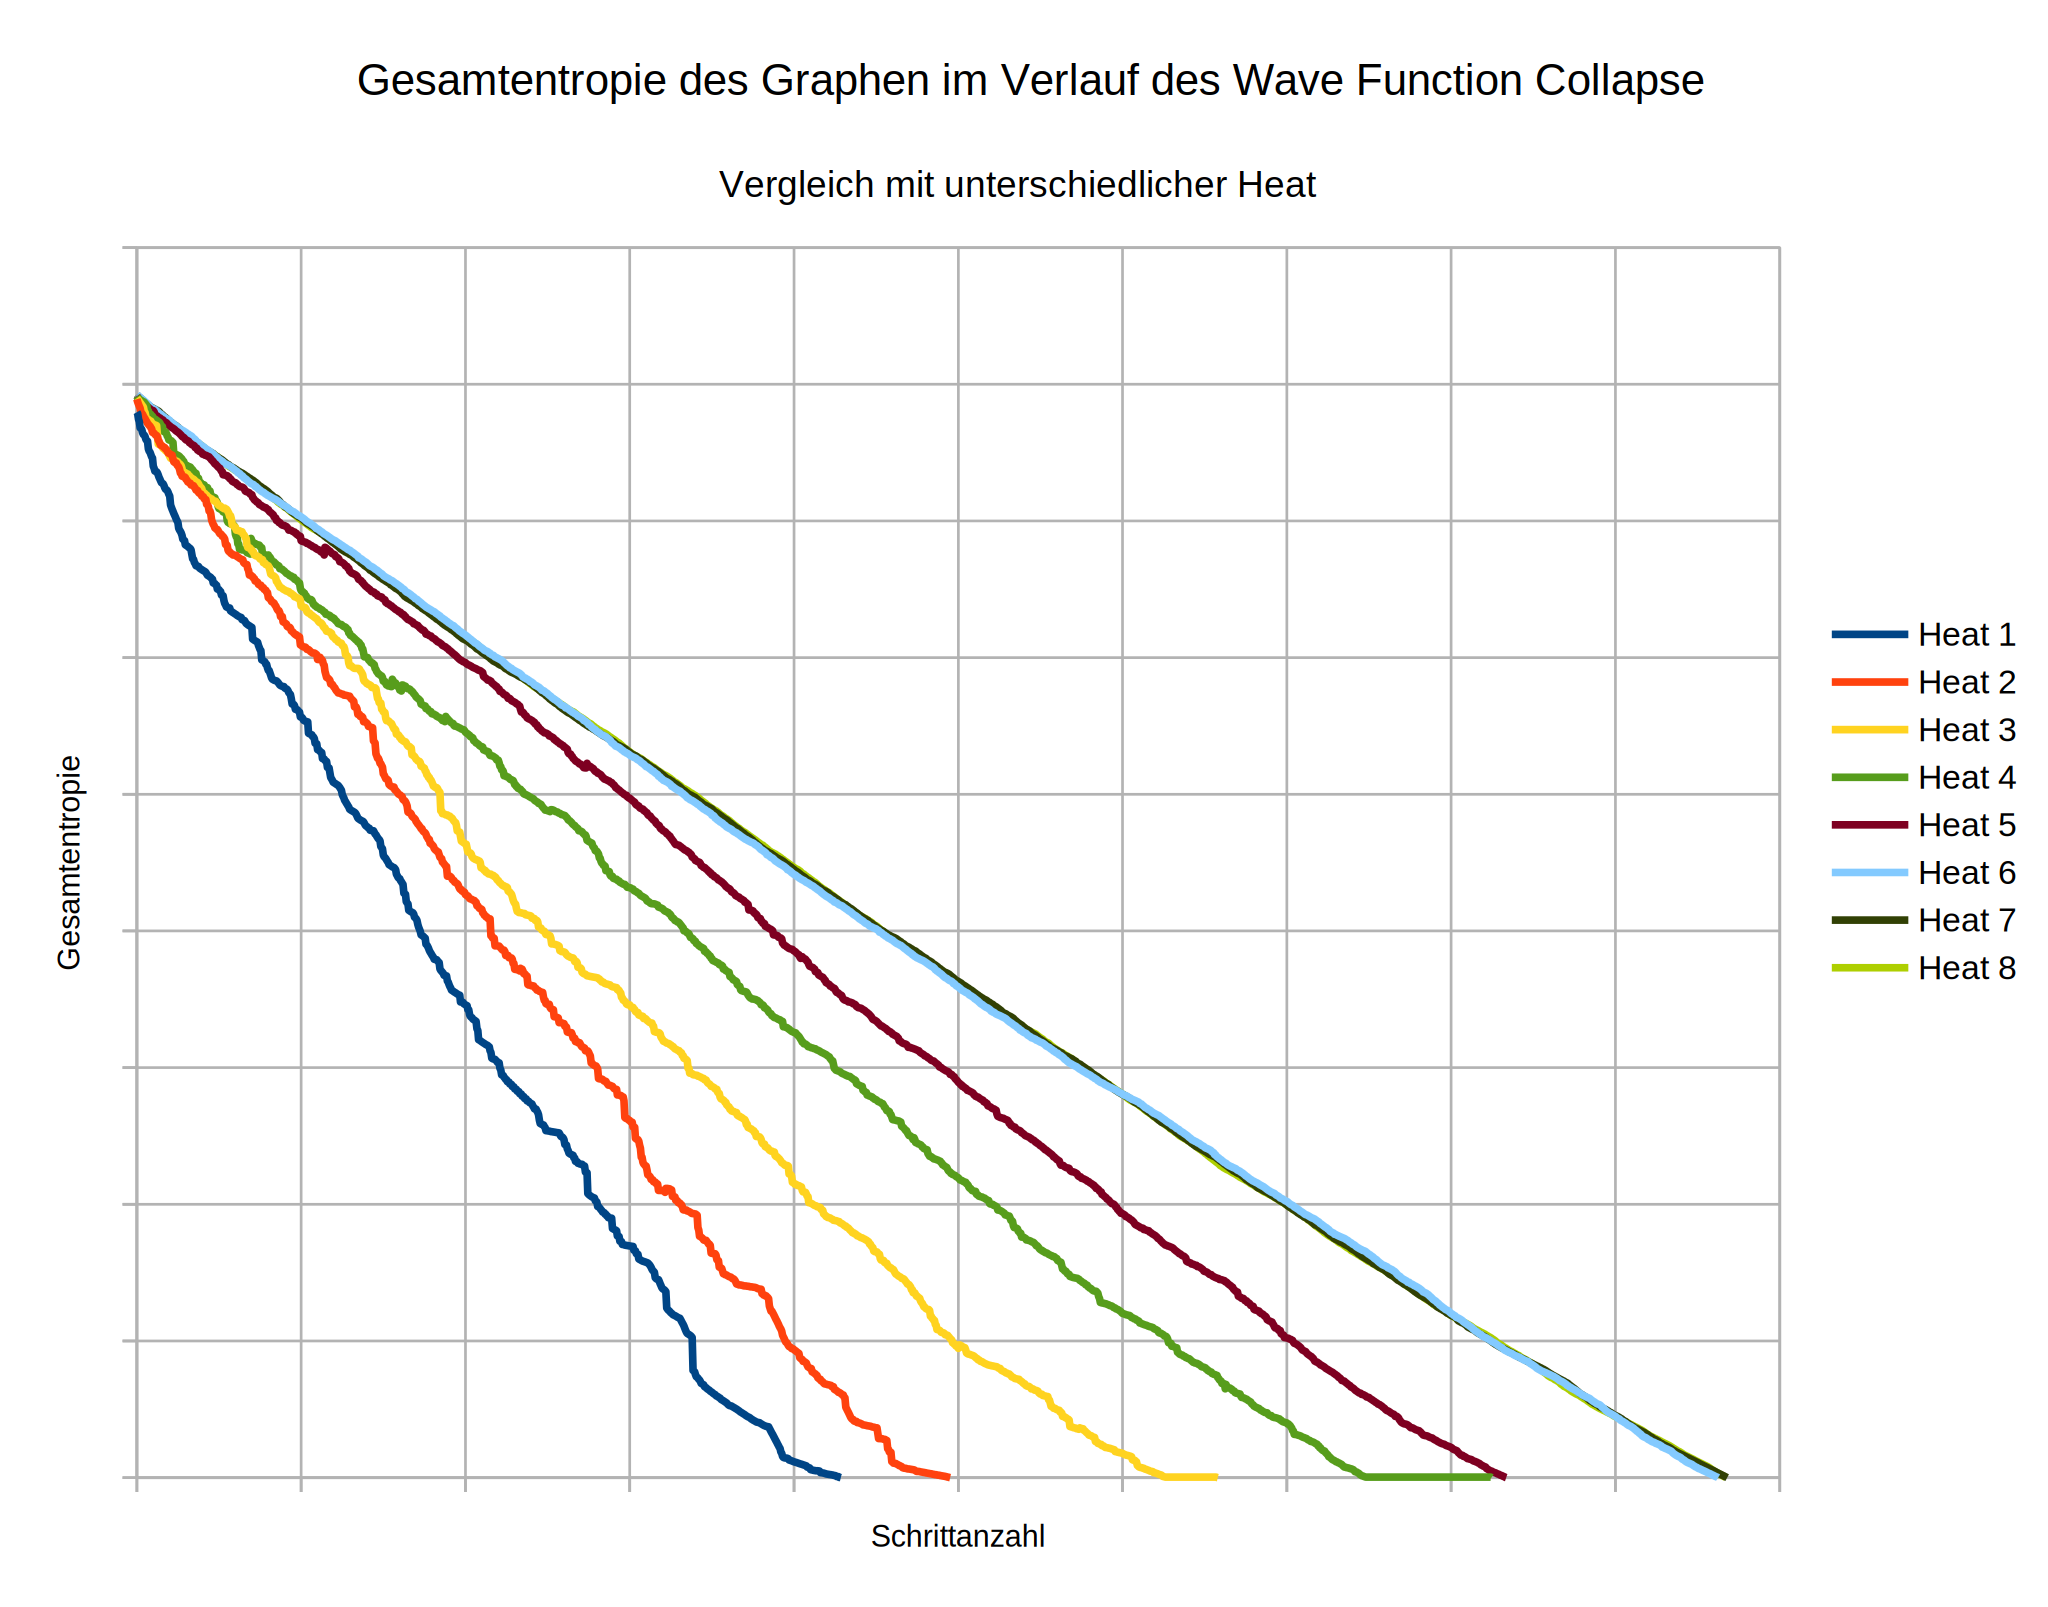
\includegraphics[width=\linewidth]{data/extract_wrapping/1.png}
        \caption{Umfeld 1}
    \end{subfigure}\hfill
    \begin{subfigure}{0.24\textwidth}
        \centering
        \includegraphics[width=\linewidth]{data/extract_wrapping/2.png}
        \caption{Umfeld 2}
    \end{subfigure}
    \begin{subfigure}{0.24\textwidth}
        \centering
        \includegraphics[width=\linewidth]{data/extract_wrapping/3.png}
        \caption{Umfeld 3}
    \end{subfigure}\hfill
    \begin{subfigure}{0.24\textwidth}
        \centering
        \includegraphics[width=\linewidth]{data/extract_wrapping/4.png}
        \caption{Umfeld 4}
    \end{subfigure}\hfill
    
    \vspace{4mm}
    
    \begin{subfigure}{0.32\textwidth}
        \centering
        \includegraphics[width=\linewidth]{data/extract_wrapping/5.png}
        \caption{Zustand 1}
    \end{subfigure}\hfill
    \begin{subfigure}{0.32\textwidth}
        \centering
        \includegraphics[width=\linewidth]{data/extract_wrapping/6.png}
        \caption{Zustand 2}
    \end{subfigure}
    \begin{subfigure}{0.32\textwidth}
        \centering
        \includegraphics[width=\linewidth]{data/extract_wrapping/7.png}
        \caption{Zustand 3}
    \end{subfigure}\hfill
    
    \caption{
        Extraktion mit vertikalem Wrapping. (a,e) Umfeld 1($U_1$) ergibt einen Zustand 1 ($Z_1$). Da die anderen Umfelder anders sind hat $Z_1$ nur eine Frequenz von 1. (d) $U_4$ überschreitet den Rand und nimmt die Pixel aus der ersten Reihe. (f) $U_2$ und $U_3$ sind gleich, darum hat $Z_2$ eine Frequenz von 2.
    }
    \label{fig:extract_wrapping}
\end{figure}